\chapter{Process Model}
\label{chap4}
A program under execution is called a process. A process is newly created when a process already in execution invokes the Fork system call. The first process, the INIT process, is created by the OS during bootstrap by loading a code stored in a pre-defined disk location to memory and setting up a process. The OS assigns a unique integer identifier called process id for each process when it is created. The process id does not change during the lifetime of the process. The process that creates the new process is called the parent process of the newly created process.
\section{The Structure of Processes}

eXpOS associates a virtual (memory) address space for each process.

\begin{figure}[ht]
\centering
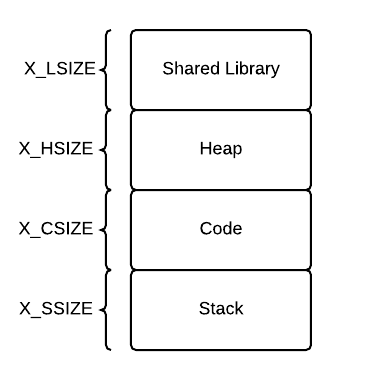
\includegraphics[scale=0.75]{figures/process_model.png}
\caption{\footnotesize Process Model in eXpOS}
\end{figure}

The address space of a process is a contiguous sequence of memory addresses, starting from zero, accessible to a process. The eXpOS logically partitions the address space into four regions library, heap, code and stack. These regions are mapped into physical memory using hardware mechanisms like paging/segmentation.


Every process corresponds to some executable file stored in XEXE format stored in the eXpFS file system. The XEXE header of the executable file contains the information about how much space must be allocated for the various memory regions. When the program is loaded into memory by the operating system, the OS reads the header and sets up the regions of the virtual address space accordingly. Once the layout of the virtual address space is clear, the OS maps the virtual address space into the physical memory. The part of the OS which does all these tasks is called the OS loader. The eXpOS loader is the interrupt service routine corresponding to the Exec system call.

A process may open files or semaphores. The OS associates a file handle with each open instance of a file. Similarly, the OS assigns a semaphore identifier (semid) for each semaphore acquired by the process. The file handles and semids acquired by a process are also attributes of a process.

Note: In addition to the above attributes of a process that are visible to application/system programs, a process under execution at any given point of time has an execution context. The context of a process refers to the contents of the registers, instruction pointer, contents of the memory etc. These are hardware dependent and are managed internally by the OS. In fact, managing the execution contexts of multiple processes simultaneously and running them all in one machine is the main challenge in the design and implementation of a multiprogramming OS. However, the OS hides these internal details from the application programs as well as system programs like compilers. 

\section{Operations on Processes}
The two most fundamental operations associated with process are Fork and Exec. The remaining operations are Exit, Wait, Signal, Getpid and Getppid.

\subsection{Semantics of Exec operation}
\begin{enumerate}
\item The OS closes all files and semaphores opened by the process. A new address space is created replacing the existing one. The new process inherits the process id of the calling process.
\item The code (and static data, if any) of the executable file are loaded into the code (and stack) regions of the new address space. The system library is mapped to the library region and stack is initialized to empty.
\item The machine instruction pointer is set to the location specified in the executable header. The machine stack pointer is initialized to the beginning of the stack. From here, execution continues with the newly loaded program.
\end{enumerate}

\subsection{Semantics of Fork operation}
\begin{enumerate}
\item A new child process with a new process id and address space is created which is an exact replica of the original process with the same library, code,stack and heap regions. (The OS assigns a new process id for the child and returns this value to the parent as the return parameter of the fork system call.) The heap, code and library regions of the parent are shared by the child. Stack is separate for the child and is not shared.
\item All open file handles and semaphores are shared by the parent and the child. This means that if one of the processes write/read into/from or adjust the file handle using the lseek system call, the corresponding file handle of the other process also gets automatically updated. Note that file handles (or semaphore identifiers) of files (or semaphores) that are opened (or created) subsequent to the fork operation by the parent or the child will be exclusive to the particular process and will not be shared. The parent and the child continue execution from here on.
\end{enumerate}

\subsection{Other Operations}
The Exit system call terminates a process after closing all files and semaphores. The Wait system call suspends the execution of a process till another process exits or executes a Signal system call. The Signal system call resumes the execution of a process that was suspended by wait.

A process can get its process id using the Getpid system call. The pid of the parent process can be obtained using the Getppid system call.

\section{Special Processes in eXpOS}
eXpOS specifies two special processes, the idle and the init process. These are stored in a predefined location in the disk and loaded to the memory by the bootstrap loader. The main purpose of idle process is to run as a background process in an infinte loop. This is demanded by the OS so that the scheduler will always have a process to schedule. The init process is the first process executed by the OS. The process identifiers for the idle and init processes are fixed as 0 and 1 respectively.

A shell is an ExpL program which takes the name of an executable file as input and executes it. The shell process Forks itself and the child process invokes the Exec system call with the executable file as argument. The shell runs until the user stops the process.
